\documentclass{article}
\usepackage {inputenc, fullpage, listings, amsmath, graphicx, amssymb, xcolor}

\parindent 0pt

\title{%
   ECE 260: Continuous-Time Signals and Systems\\
    \Large Alex Holland\\
    Assignment 3B\\
    }
\date{}

\begin{document}

\maketitle


4.11 {\bf [find impulse response]}\\
(a)\\
\begin{equation*}
\begin{split}
    \mathcal{H}x(t) &= \int_{-\infty}^{t + 1} x(\tau)d\tau, \; x(\tau) = \delta(\tau)\\
    h(t) &= \int_{-\infty}^{t + 1} \delta(\tau)d\tau\\
    &= \begin{cases}
        1 & t > -1\\
        0 & t < -1\\
    \end{cases}\\
    &= u(t + 1)
\end{split}
\end{equation*}

(b)\\
\begin{equation*}
\begin{split}
    \mathcal{H}x(t) &= \int_{-\infty}^{\infty} x(\tau + 5)e^{\tau - t + 1}u(t - \tau - 2)d\tau\\\\
    x(\tau) &= \delta(\tau)\\
    \tau + 5 &= 0\\
    \tau &= -5\\\\
    h(t) &= \int_{-\infty}^{\infty} \delta(\tau + 5)e^{\tau - t + 1}u(t - \tau - 2)d\tau\\
    &= e^{-5 - t + 1}u(t - (-5) - 2)\\
    &= e^{-(t + 4)}u(t + 3)\\
\end{split}
\end{equation*}

(c)\\
\begin{equation*}
\begin{split}
    \mathcal{H}x(t) &= \int_{-\infty}^{t} x(\tau)v(t - \tau)d\tau\\\\
    h(t) &= \int_{-\infty}^{t} \delta(\tau)v(t - \tau)d\tau\\
    \lambda &= \tau - t\\
    \tau &= \lambda + t\\
    \tau &= d\lambda\\\\
    h(t) &= \int_{-\infty}^{0} \delta(\lambda + t)v(t - (\lambda + t))d\lambda\\
    &= \int_{-\infty}^{0} \delta(\lambda + t)v(-\lambda)d\lambda\\
    &= \int_{-\infty}^{0} \delta(\lambda + t)v(t)d\lambda\\
    &= v(t) \int_{-\infty}^{0} \delta(\lambda + t)d\lambda\\
    &= v(t)u(t)\\
\end{split}
\end{equation*}

\bigskip
4.12 {\bf [impulse response and series/parallel interconnection]}\\
(a)\\
\begin{equation*}
\begin{split}
    v(t) &= x * h_1(t)\\
    y(t) &= v * [h_2 + h_3](t) + x(t)\\
\end{split}
\end{equation*}

Combining the results we get:

\begin{equation*}
\begin{split}
    y(t) &= v * [h_2 + h_3](t) + x(t)\\
    &= [x * h_1] * [h_2 + h_3](t) + x(t)\\
    &= [h_1 * [h_2 + h_3]](t) + x(t)\\
    &= x * [h_1 * h_2 + h_1 * h_3](t) + x * \delta(t)\\
    &= x * [h_1 * h_2 + h_1 * h_3 + \delta](t)\\
\end{split}
\end{equation*}

Thus:

\begin{equation*}
\begin{split}
    h(t) &= h_1 * h_2(t) + h_1 * h_3(t) + \delta(t)
\end{split}
\end{equation*}

(b)\\
We want to determine the impulse response $h$ in the specific case that:
\begin{equation*}
\begin{split}
    h_1(t) = \delta(t + 1), \; h_2(t) = \delta(t), \; h_3(t) = \delta(t)\\
\end{split}
\end{equation*}
\begin{equation*}
\begin{split}
    h_1(t)& = \delta(t + 1), h_2(t) = \delta(t), \text{ and } h_3(t) = \delta(t)\\
    h(t) &= h_1 * h_2(t) + h_1 * h_3(t) + \delta(t)\\\\
    h(t) &= \delta(t + 1) * \delta(t) + \delta(t + 1) * \delta(t) + \delta(t)\\
    &= \delta(t + 1) + \delta(t + 1) + \delta(t)\\
    &= 2 \delta(t + 1) + \delta(t)\\
\end{split}
\end{equation*}

\bigskip
4.13 {\bf [convolution, impulse response, system interconnection]}\\
(b)\\
\begin{equation*}
\begin{split}
    h_1(t) = \delta(t + 1) \text{ and } h_2(t) = \delta(t + 1)\\
\end{split}
\end{equation*}
\begin{equation*}
\begin{split}
    h(t) &= h_1 * h_2\\
    &= \delta (t + 1) + \delta(t + 1)\\
    &= \int_{-\infty}^{\infty} \delta(\tau + 1) \delta(t - \tau + 1)d \tau\\
    &= \delta(t - \tau + 1)\big|_{\tau = -1}\\
    &= \delta(t - (-1) + 1)\\
    &= \delta(t + 2)\\\\
    y(t) &= x * h(t)\\
    &= u(t) * \delta(t + 2)\\
    &=  \int_{-\infty}^{\infty} u(\tau) \delta(t - \tau + 2)d\tau\\
    &= u(\tau)\big|_{\tau = t + 2}\\
    &= u(t + 2)\\
\end{split}
\end{equation*}

(c)\\
\begin{equation*}
\begin{split}
    h_1(t) &= e^{-3t}u(t) \text{ and } h_2(t) = \delta(t)\\\\
    h(t) &= h_1(t) * h_2(t), \;\; t - \tau = 0, \; t = \tau\\
    &= e^{-3t}u(t) * \delta(t)\\
    &= \int_{-\infty}^{\infty} e^{-3t}u(\tau) \delta(t - \tau)d\tau\\
    &= e^{-3t}u(t)\\
\end{split}
\end{equation*}

We want to consider $y(t)$ at  $t < 0$ and $t \geq 0$. For $t \geq 0$:
\begin{equation*}
\begin{split}
    y(t) &= x * h(t)\\
    &= h * x(t)\\
    &= \int_{-\infty}^{\infty} e^{-3\tau}u(\tau) u(t - \tau)d\tau\\
    &= \int_{0}^{t} e^{-3\tau}d\tau\\
    &= -\frac{1}{3}e^{-3\tau}\big|_0^t\\
    &= -\frac{1}{3}e^{-3t} + \frac{1}{3}\\
\end{split}
\end{equation*}

When $t < 0$, $y(t)$ is $0$, so the convolution of $y(t)$ can be represented as:
\begin{equation*}
\begin{split}
    y(t)
    &= \begin{cases}
        -\frac{1}{3}e^{-3t} + \frac{1}{3} & t \geq 0\\
        0 & t < 0\\
    \end{cases}\\
    &= [-\frac{1}{3}e^{-3t} + \frac{1}{3}]u(t)
\end{split}
\end{equation*}


\bigskip
4.14 {\bf [causality, memory]}\\
(a)\\
\begin{equation*}
\begin{split}
    h(t) &= (t + 1) u (t - 1)\\
    u(t - 1)
    &= \begin{cases}
        1 & t \geq 1\\
        0 & t < 1\\
    \end{cases}\\
    h(t) &= 0, \; t < 0
\end{split}
\end{equation*}
Since $h(t) \neq 0$ for all $t \neq 0$, and $h(t) = 0$ for all $t < 0$, the system is causal and has memory

\smallskip
(f)\\
\begin{equation*}
\begin{split}
    h(t) &= e^{-3|t|}\\
    & e^{-3|t|}, \; -\infty < t < \infty\\
\end{split}
\end{equation*}
Since $h(t) \neq 0$ for all $t \neq 0$, and $h(t) \neq 0$ for all $t < 0$, the system has memory but is not causal.

\smallskip
(g)\\
\begin{equation*}
\begin{split}
    h (t) &= 3\delta(t)\\
    t\delta(t)
    &= \begin{cases}
        3 & t = 0\\
        0 & t \neq 0\\
    \end{cases}\\
\end{split}
\end{equation*}
Since $h(t) = 0$ for all $t \neq 0$, and $h(t) = 0$ for all $t < 0$, the system is memoryless and causal.


\break
4.15 {\bf [BIBO stability]}\\
(a)\\
\begin{equation*}
\begin{split}
    u &= at\\
    \frac{du}{dt} &= a\\
    \frac{1}{a}du &= dt\\\\
     \int_{-\infty}^{\infty} |h(t)|dt &= \int_{-\infty}^{\infty} |e^{at}u(-t)|dt\\
     &= \int_{-\infty}^{0} e^{at}dt\\
     &= [\frac{1}{a}e^{at}]\big|_{-\infty}^0\\
     &= \frac{1}{a}[e^{at}]\big|_{-\infty}^0\\
     &= \frac{1}{a}[e^{a+0} - e^{a(-\infty)}]\\
     &= \frac{1}{a}[1 - 0]\\
     &= \frac{1}{a}\\
     & \text{which is $< \infty$}\\
\end{split}
\end{equation*}
$\therefore$ the system is BIBO stable

\smallskip
(b)\\
\begin{equation*}
\begin{split}
    h(t) = \frac{1}{t}u(t - 1\\
    \int_{-\infty}^{\infty}|h(t)| &= \int_{-\infty}^{\infty}|\frac{1}{t}u(t - 1)|dt\\
    &= \int_{-\infty}^{1}0dt + \int_{1}^{\infty}\frac{1}{t}dt\\
    &= \int_{1}^{\infty} \frac{1}{t}dt\\
    &= [lnt]\big|_1^{\infty}\\
    &= ln \infty - ln1\\
    &= \infty\\
\end{split}
\end{equation*}
$\therefore$ the system is not BIBO stable


\bigskip
4.16 {\bf [inverse system]}\\
$h_1(t) = \frac{1}{2}\delta(t - 1), \; h_2(t) = 2\delta(t + 1)$. We can determine if the systems are inverses if $h_1(t) * h_2(t) = \delta(t)$.
\begin{equation*}
\begin{split}
    h_1 * h_2(t) &=  \int_{-\infty}^{\infty} h_1(\tau) h_2(t - \tau)d\tau\\
    &= \int_{-\infty}^{\infty} \frac{1}{2} \delta(\tau - 1) 2\delta(t - \tau + 1)d\tau\\
    &= \int_{-\infty}^{\infty} \delta(\tau - 1) \delta(t - \tau + 1) d\tau, \; t - \tau + 1 = 0, \; \tau = t + 1\\
    &= \delta(\tau - 1)\big|_{\tau = t + 1}\\
    &= \delta(t + 1 - 1)\\
    &= \delta(t)\\
\end{split}
\end{equation*}
$\therefore$ the systems are inverses of each other

\bigskip
4.17 {\bf [system function, eigenfunction]}\\
(a)\\
We want to find the response $y$ of the LTI system with system function $H$ to the input $x$.
\begin{equation*}
\begin{split}
    h(s) = \frac{1}{s + 1} \text{ for } Re(s) > -1 \text{ and } x(t) = 10 + 4cos(3t) + 2sin(5t)
\end{split}
\end{equation*}
Knowing that $ae^{j\theta} + a^*e^{-j\theta} = 2Re(ae^{j\theta})$ we can determine x(t):
\begin{equation*}
\begin{split}
    x(t) &= 10 + 4[\frac{1}{2}(e^{j3t} + e^{-j3t})] + 2[\frac{1}{2j}(e^{j5t} - e^{-j5t})]\\
    &= 10 + 2(e^{j3t} + e^{-j3t}) + \frac{1}{j}(e^{j5t} - e^{-j5t})\\
    &= 10 + 2e^{j3t} + 2e^{-j3t} - je^{j5t} + je^{-j5t}
\end{split}
\end{equation*}
We have an LTI system with system function $H$ to the input $x$, so:
\begin{equation*}
\begin{split}
    y(t) &= H(0)(10) + H(j3)(2e^{j3t}) + H(-j3)(2e^{-j3t}) + H(j5)(-je^{j5t}) + H(-j5)(je^{-j5t})\\
    &= 1(10) + \frac{1}{1 + j3}(2e^{j3t}) + \frac{1}{1 - j3}(2e^{-j3t}) + \frac{1}{1 + j5}(-je^{j5t}) + \frac{1}{1 - j4}(je^{-j5t})\\
    &= 10 + \frac{2}{1 + j3}e^{j3t} + (\frac{2}{1 + j3})^*(e^{j3t})^* + ^*(\frac{-j}{1 + j5})^*(e^{j5t})^*\\
    & \text{Since } ae^{j\theta} + a^*e^{-j\theta} = 2Re(ae^{j\theta}) \text{ we get:}\\
    &= 10 + 2Re(\frac{2}{1 + j3}e^{j3t}) + 2 Re(\frac{-j}{1 + j5}e^{j5t})\\
\end{split}
\end{equation*}


\break
D.108 {\bf [graphic patterns]}\\
(a)
\begin{lstlisting}
    function drawpattern(n, theta)
        angle = theta * (pi / 180);
        p = [0 0]'; 
        prime = p';
        m = [cos(angle) sin(angle); -sin(angle) cos(angle)];
        for i = 1 : (n - 1)
            p = p + m ^ (i - 1) * [i 0]';
            prime = [prime; p'];
        end
        plot(prime(:, 1), prime(:, 2));
        axis('equal');
    end
\end{lstlisting}

(b)\\\
$n = 100$ and $\theta = 89$
\begin{center}
    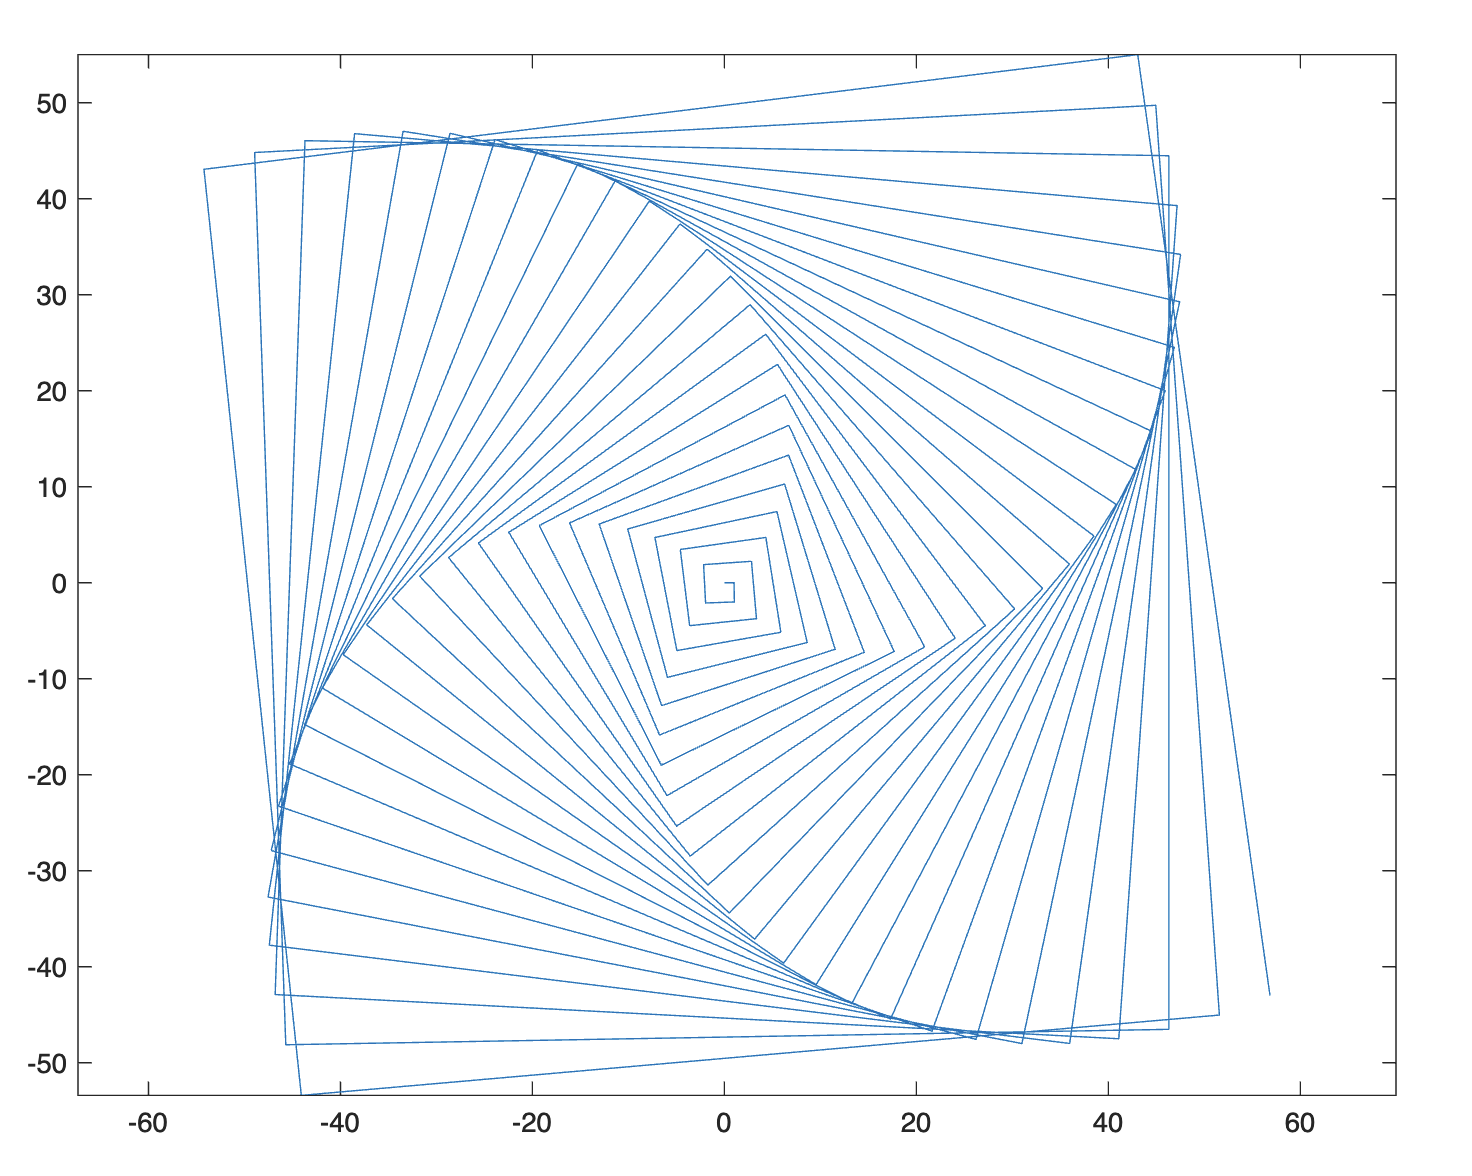
\includegraphics[width=0.6\textwidth]{108b1.png}
\end{center}
$n = 100$ and $\theta = 144$
\begin{center}
    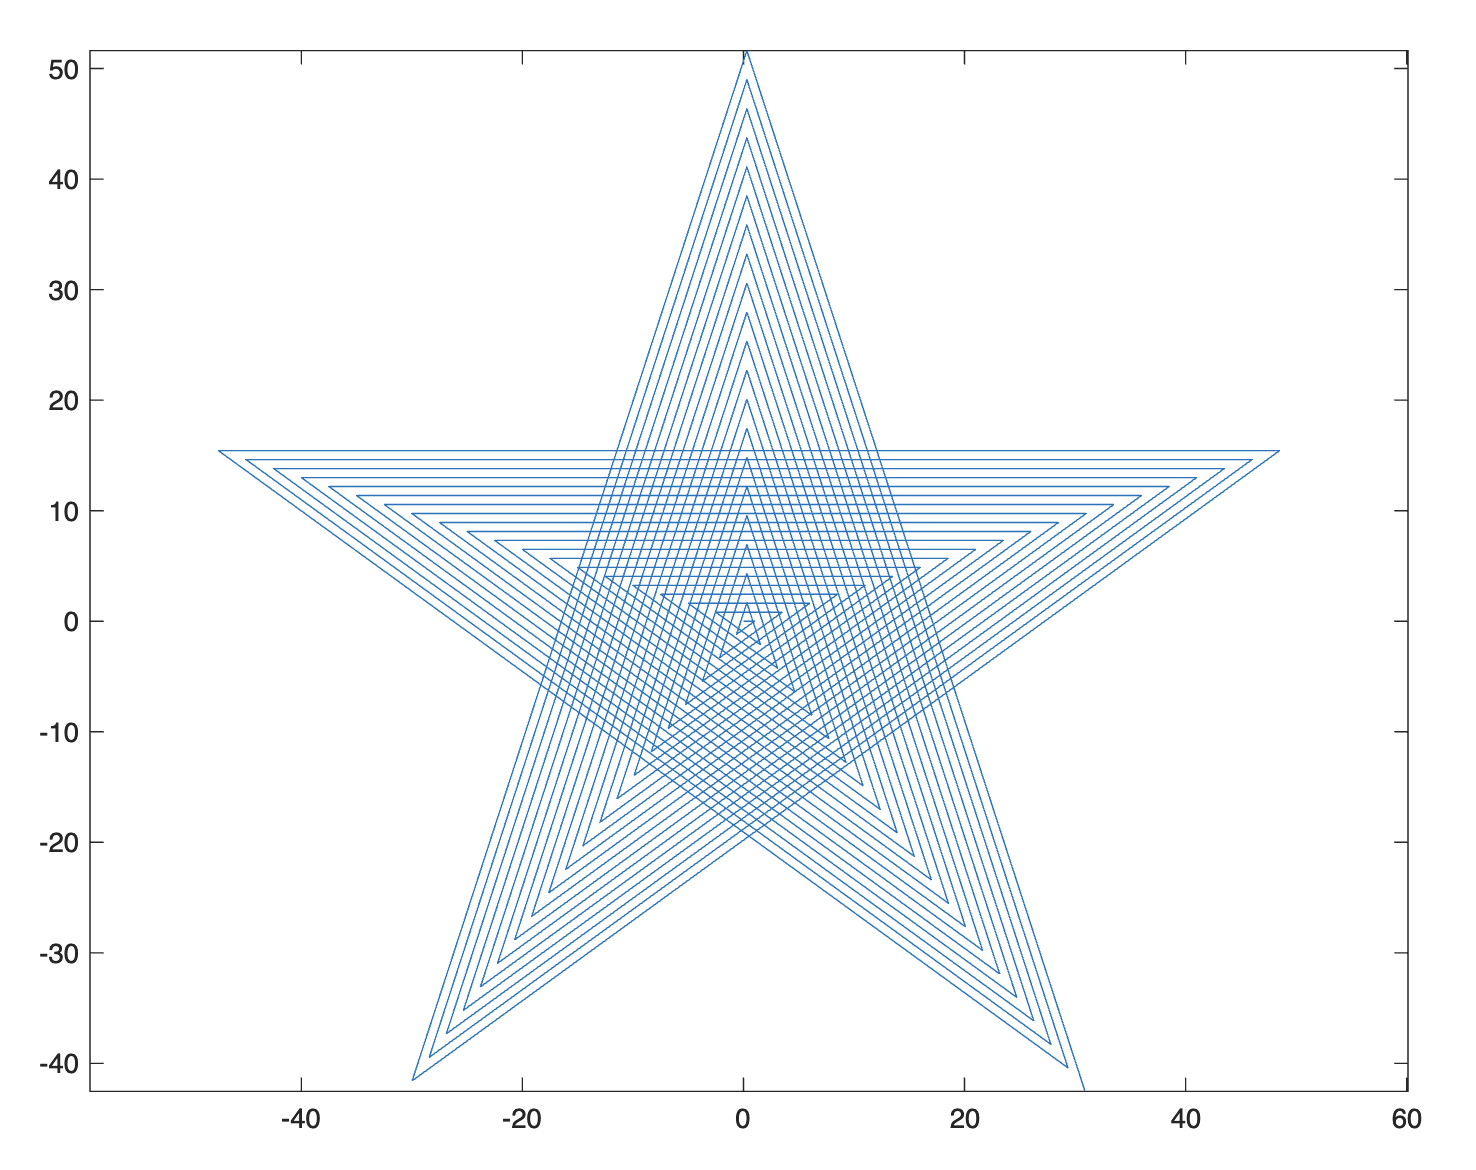
\includegraphics[width=0.6\textwidth]{108b2.png}
\end{center}
$n = 100$ and $\theta = 154$
\begin{center}
    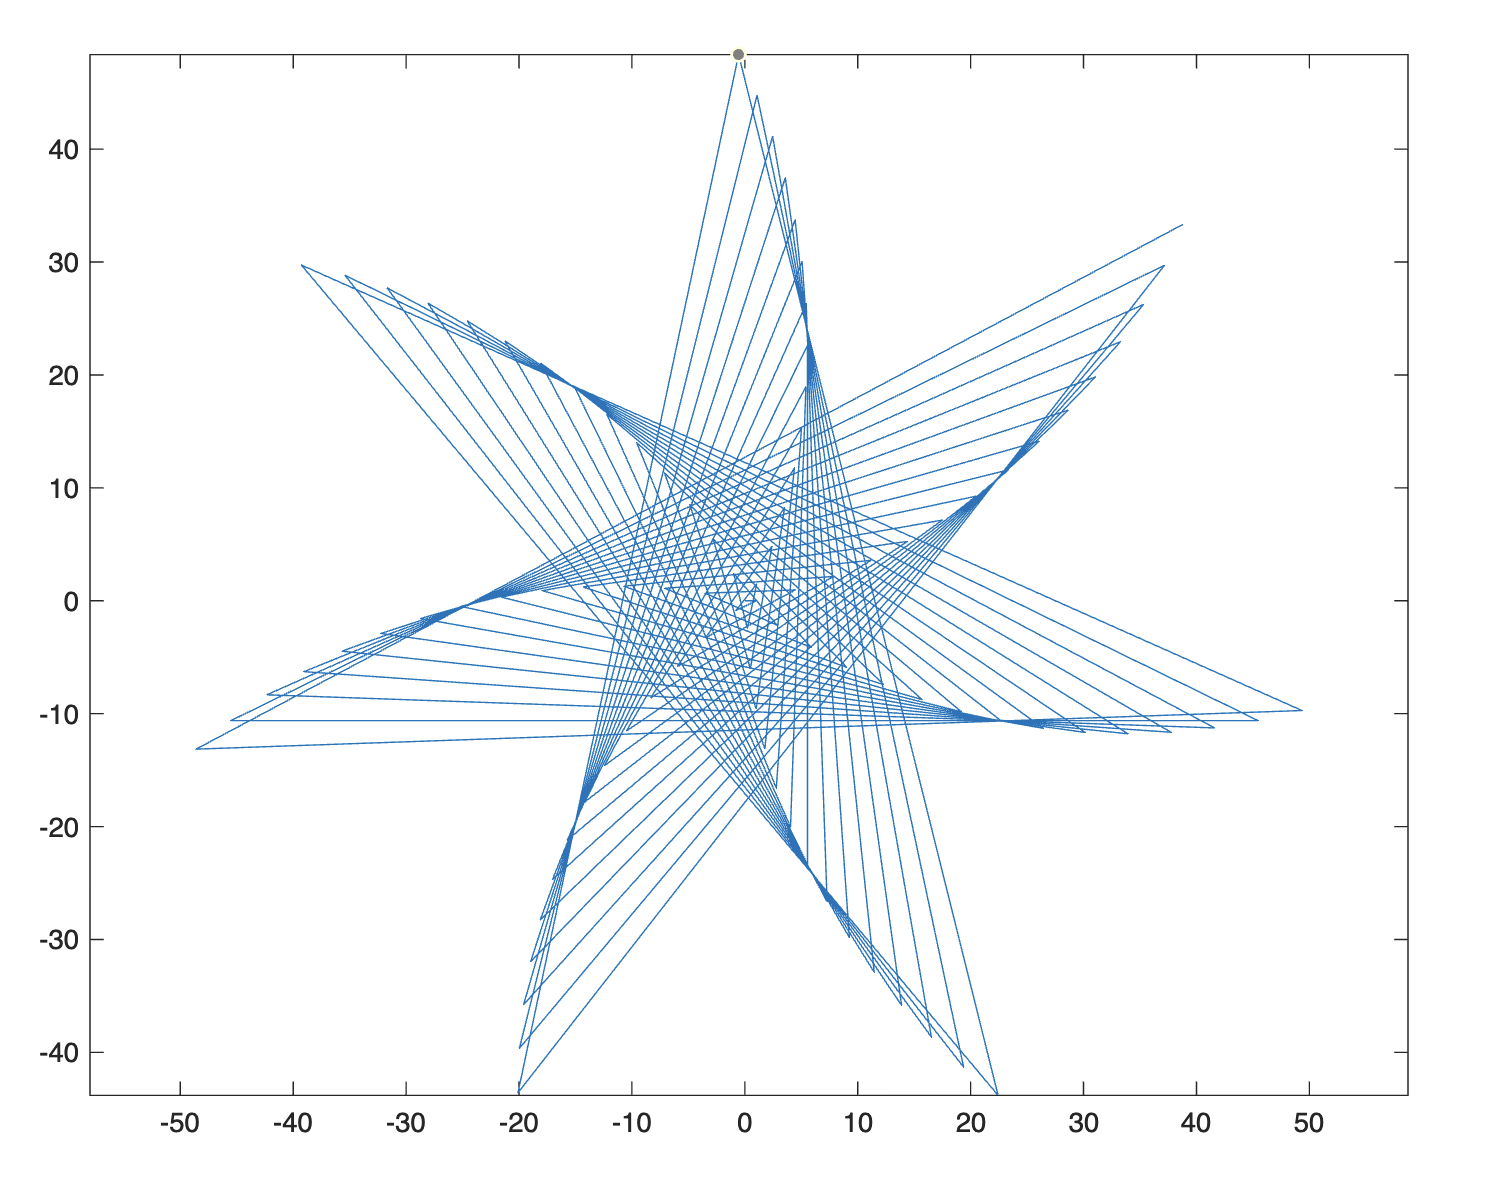
\includegraphics[width=0.6\textwidth]{108b3.png}
\end{center}


\end{document}
